%\documentclass[twocolumn,10pt]{jarticle} 
\documentclass[10pt]{jarticle} 
%
\usepackage{listings,jlisting}
\usepackage{amsmath,amssymb}
\usepackage{bm}
\usepackage{ascmac}
\usepackage[dvipdfmx]{graphicx}
\usepackage{here}
\usepackage{comment}
%
%ここからソースコードの表示に関する設定
\lstset{
  basicstyle={\ttfamily},
  identifierstyle={\small},
  commentstyle={\smallitshape},
  keywordstyle={\small\bfseries},
  ndkeywordstyle={\small},
  stringstyle={\small\ttfamily},
  frame={tb},
  breaklines=true,
  columns=[l]{fullflexible},
  numbers=left,
  xrightmargin=0zw,
  xleftmargin=3zw,
  numberstyle={\scriptsize},
  stepnumber=1,
  numbersep=1zw,
  lineskip=-0.5ex
}
%ここまでソースコードの表示に関する設定
%
%画像の貼り方
\begin{comment}
\begin{figure}[H]
  \begin{center}
  \includegraphics[width=10cm]{arm/fig3.png}
  \caption{ロボットアームのシミュレーションの様子1}
  \end{center}
\end{figure}
\end{comment}
%
\title{数理実習B(離散手法)レポート}
\author{学生証番号:03-190615\\氏名:工藤龍\\メールアドレス:ron233f@gmail.com}
\date{\today}
%
\begin{document}
\maketitle

\section{概要}
研究室のホームページの役割には様々なものがある.
その中でも重要なものが,これから研究室を決める学生や,
共同研究先を探している企業の人などが見る場合である.
そのような人たちが求めているものは,
研究室がどのような研究をしていて,どんな人が所属しているかなどの
基本的な情報を素早くわかりやすい形で入手することである.

これを鑑みると,この目的における「より良い」ウェブサイトとは,
余分な情報はあまり含まず,重要な情報がアクセスしやすいサイトである
ということができる.

今回の解析では,
計数工学科システム情報工学コースの8個の研究室を比較し,
どの研究室のウェブサイトがより理想的な形になっているかを考察した.

\section{解析手法}
各研究室の全てのページに関してそれぞれのサイト内でのページランクを算出した.
その後,それをヒストグラムとして可視化し,それぞれのサイトの
特徴を考察した.ページランク算出の際のダンピング係数は0.85とした.

\section{結果}
ページランクを各研究室のウェブサイトの全てのページについて算出した結果,
次の図1から図8までのヒストグラムのようになった.

\begin{figure}[H]
  \begin{center}
  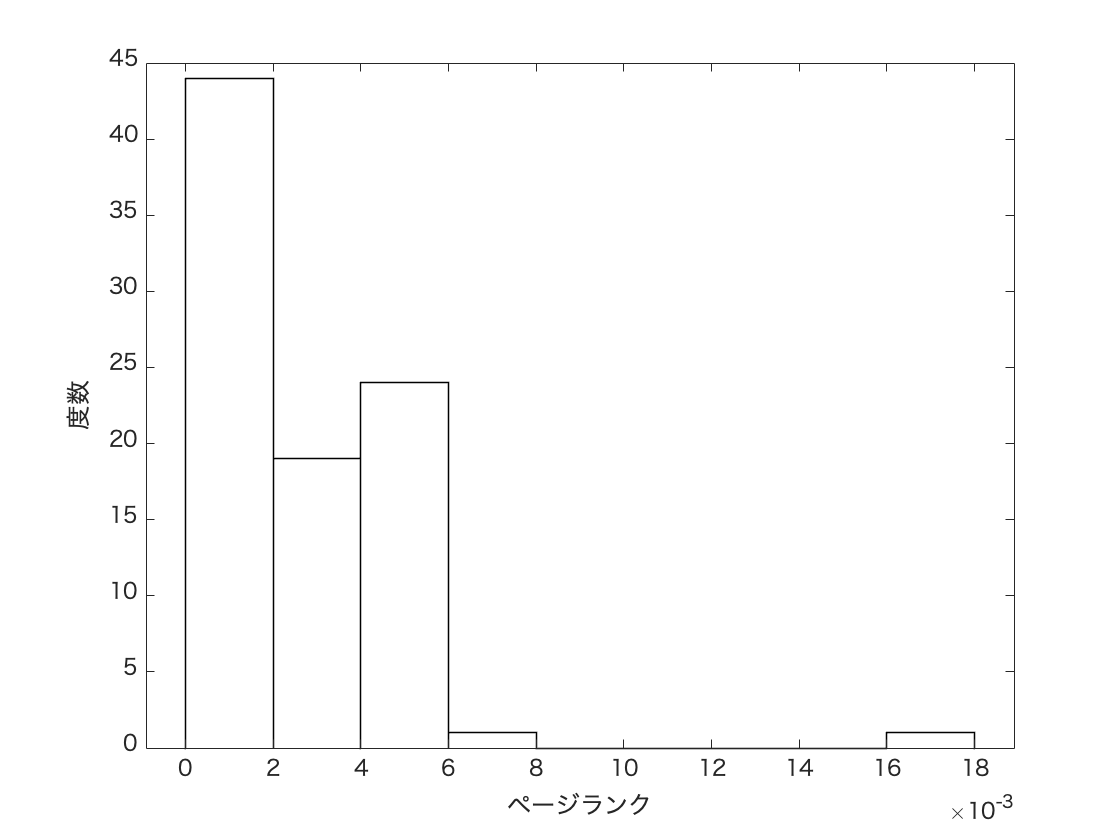
\includegraphics[width=10cm]{../histograms/i1.png}
  \caption{第1研究室のページランクの分布}
  \end{center}
\end{figure}

\begin{figure}[H]
  \begin{center}
  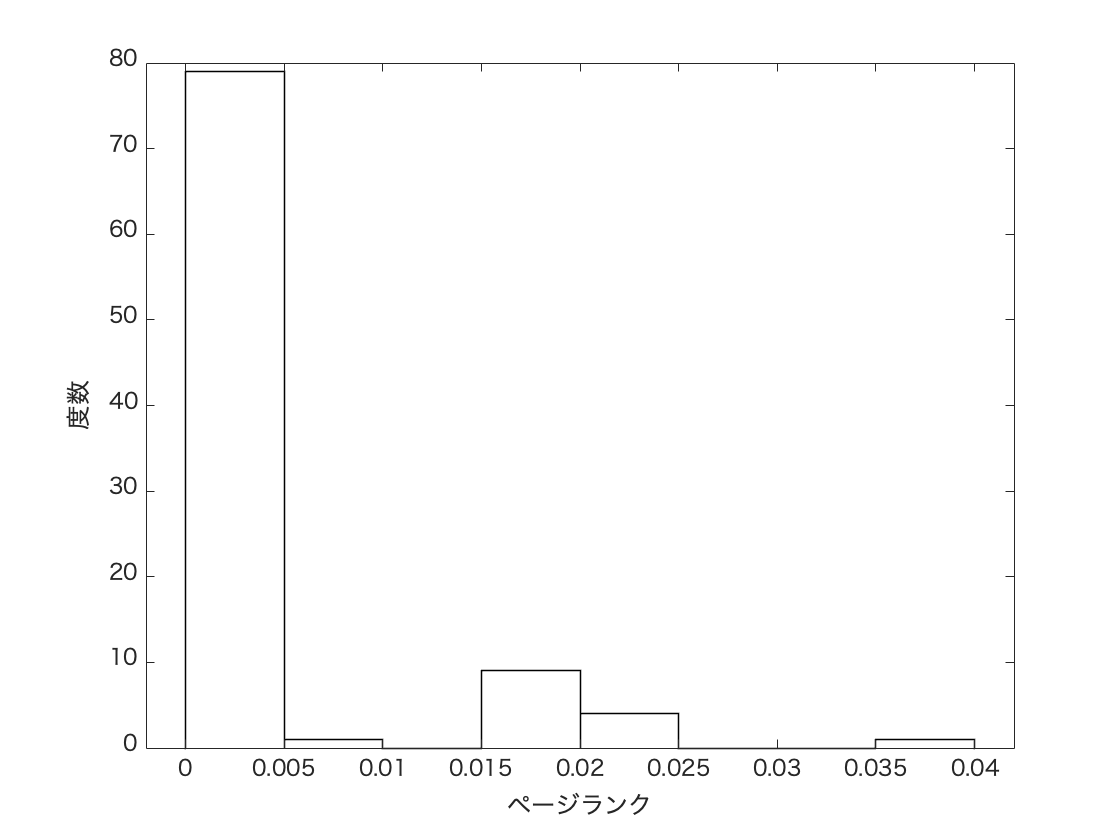
\includegraphics[width=10cm]{../histograms/i2.png}
  \caption{第2研究室のページランクの分布}
  \end{center}
\end{figure}

\begin{figure}[H]
  \begin{center}
  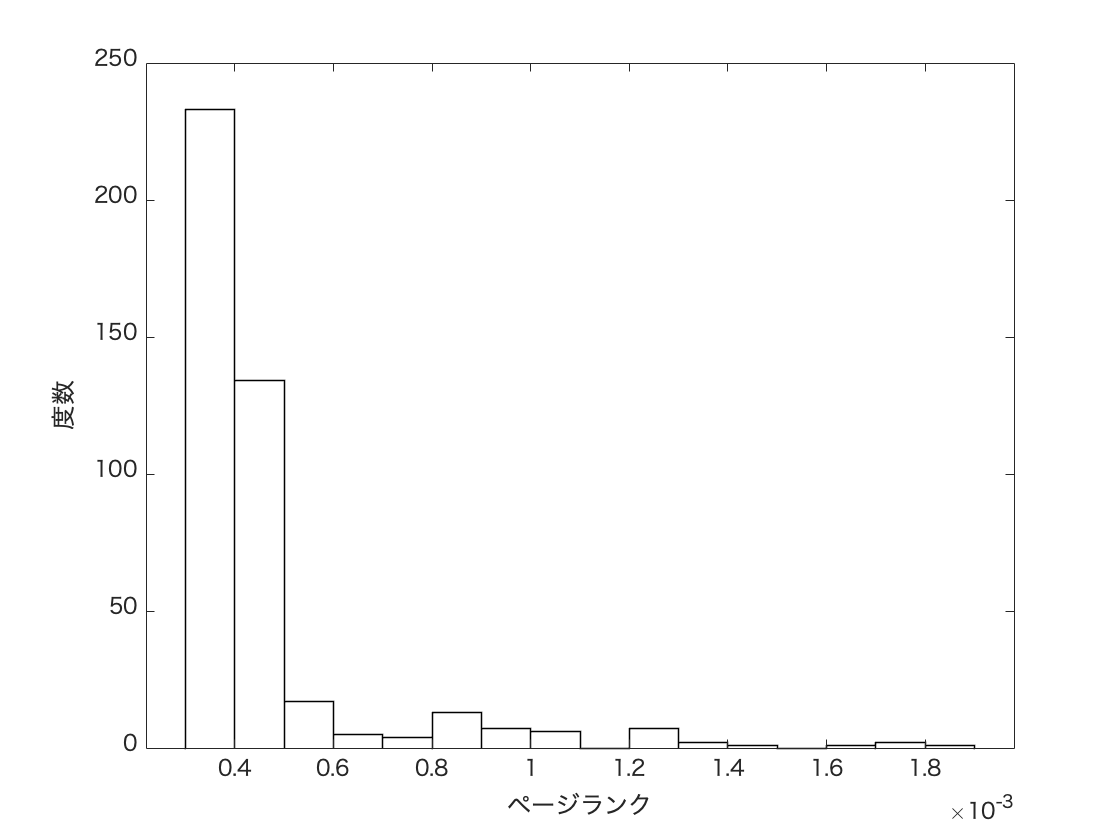
\includegraphics[width=10cm]{../histograms/i3.png}
  \caption{第3研究室のページランクの分布}
  \end{center}
\end{figure}

\begin{figure}[H]
  \begin{center}
  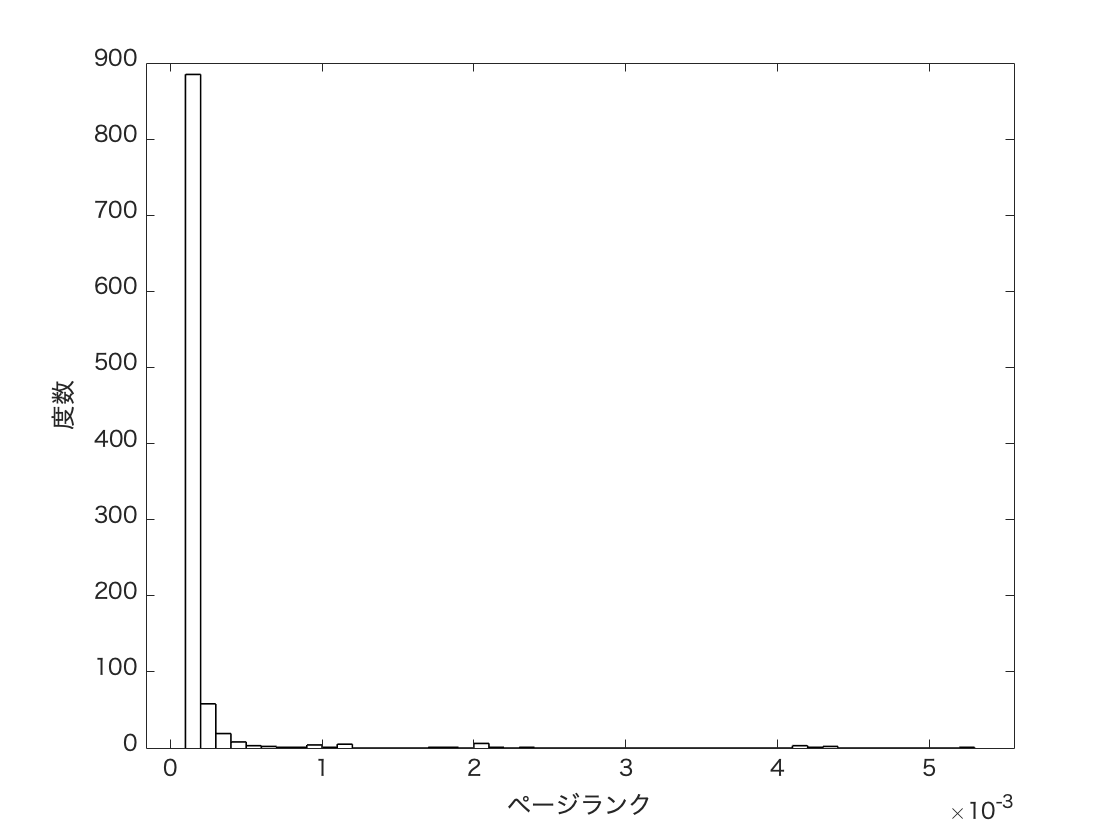
\includegraphics[width=10cm]{../histograms/i4.png}
  \caption{第4研究室のページランクの分布}
  \end{center}
\end{figure}

\begin{figure}[H]
  \begin{center}
  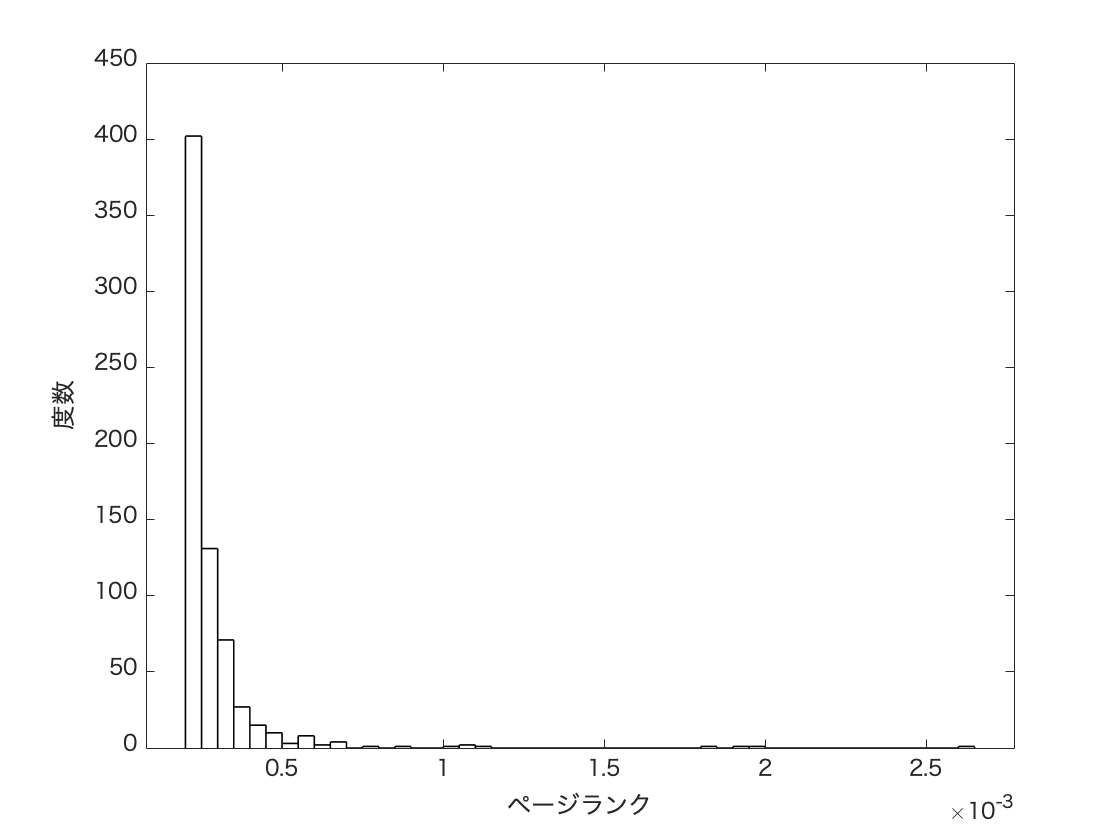
\includegraphics[width=10cm]{../histograms/i5.png}
  \caption{第5研究室のページランクの分布}
  \end{center}
\end{figure}

\begin{figure}[H]
  \begin{center}
  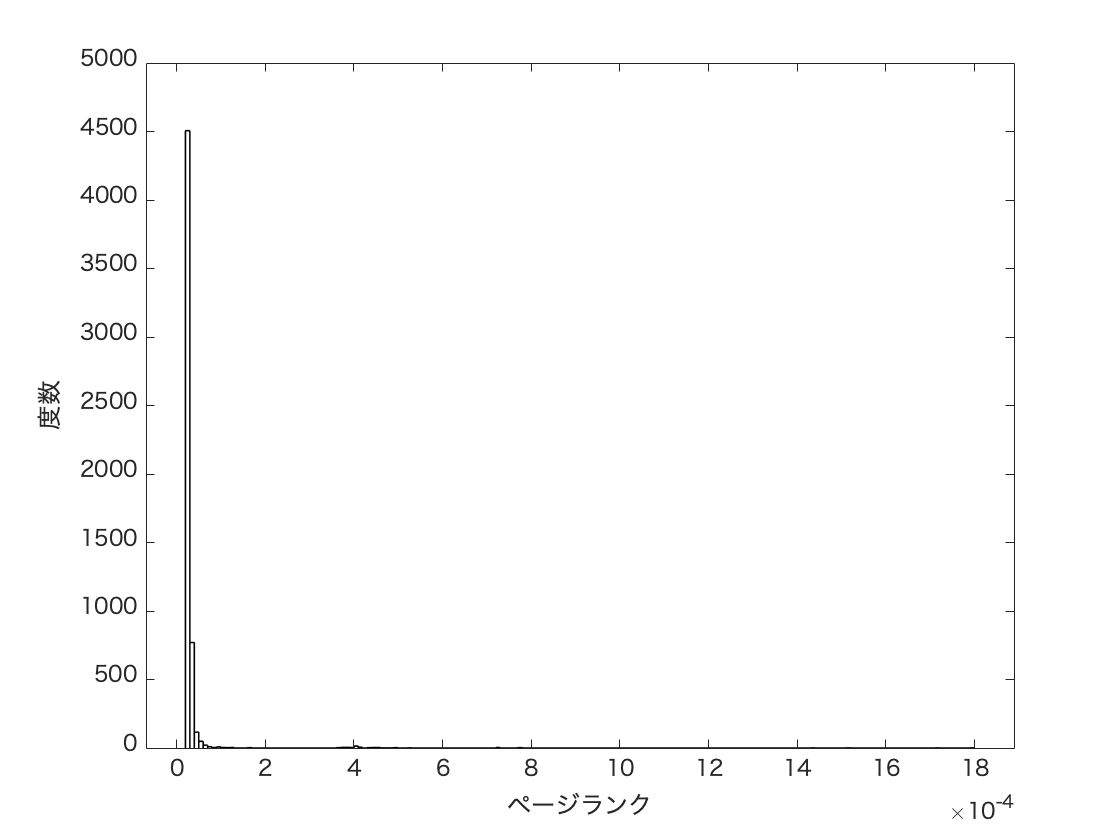
\includegraphics[width=10cm]{../histograms/i6.png}
  \caption{第6研究室のページランクの分布}
  \end{center}
\end{figure}

\begin{figure}[H]
  \begin{center}
  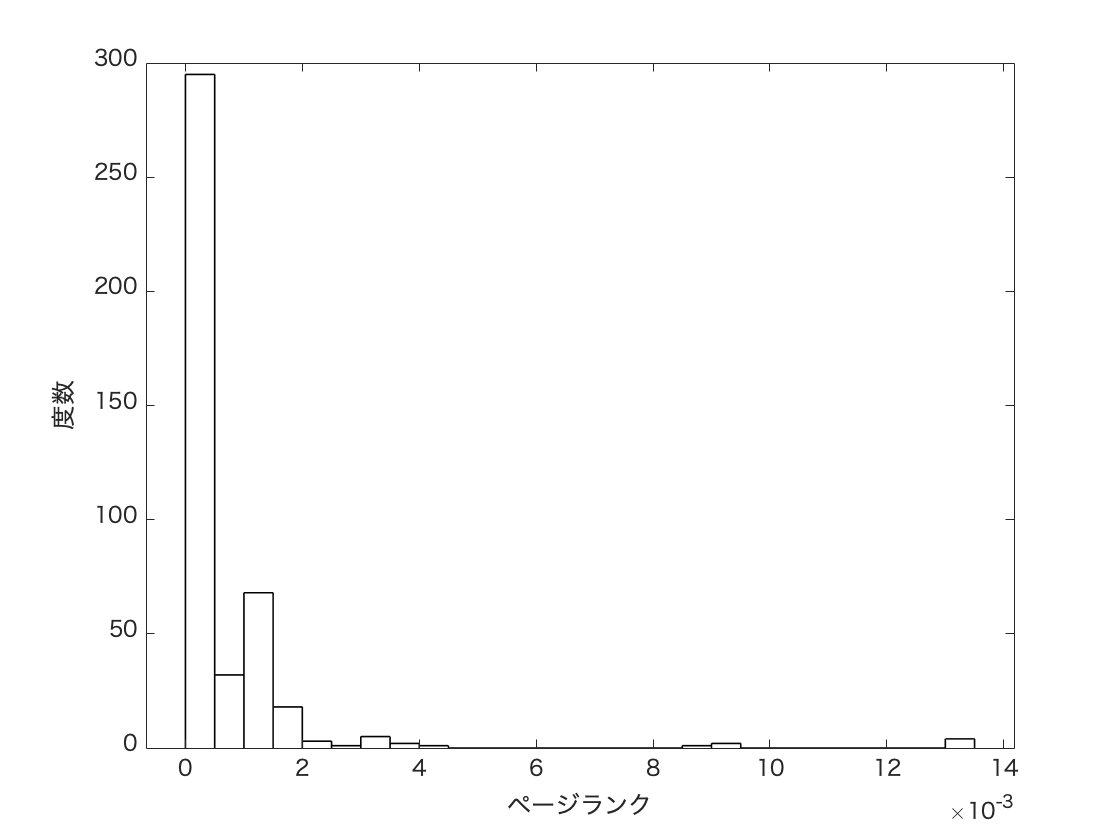
\includegraphics[width=10cm]{../histograms/i7.png}
  \caption{第7研究室のページランクの分布}
  \end{center}
\end{figure}

\begin{figure}[H]
  \begin{center}
  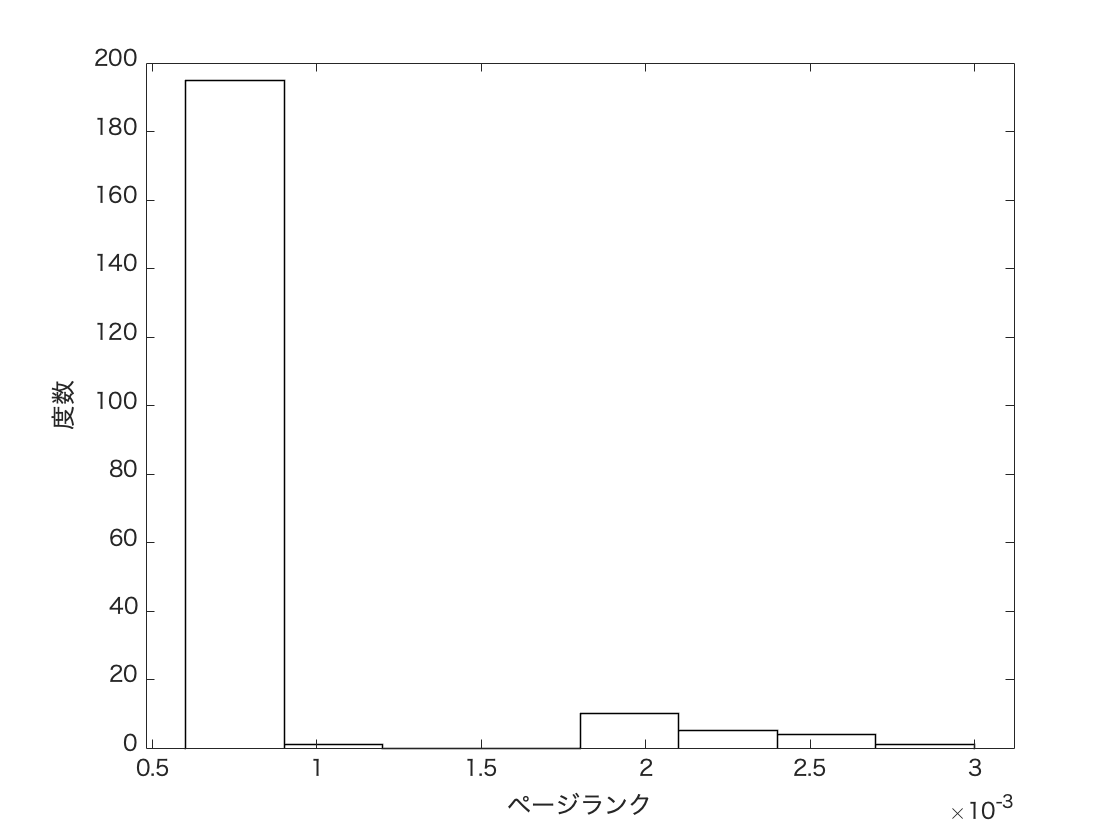
\includegraphics[width=10cm]{../histograms/ia.png}
  \caption{先端研生田研究室のページランクの分布}
  \end{center}
\end{figure}

\section{考察}

ヒストグラムを全体としてみると,まずわかることとして
研究室によってヒストグラムの形状が全く異なることがあげられる.
ページランクの低いものがどのサイトも多くなっている点では共通しているが,
その割合は大きく異なっている.
研究室ごとにコンテンツの加え方・記載している情報と捨象している情報などの
運用方針が異なることが推察される.

第2研究室を見ると,ページランク最大のもののページランクが唯一
0.35を超えていることがわかる.これは,ある一つのページに
多くのリンクが繋がっていて,かつそのページから多くの
ページにリンクが繋がっていることを意味する.
相対的にページランクが小さいものの割合が小さいため,
重要な情報がまとまっていると予想される.ゆえに
学生や企業の人にとっては「良い」サイトと言えるだろう.

また,もう一つ特徴的な研究室が第6研究室である.
ここは,ページランクの小さいものの数が異常に多く,
相対的にページランクが大きいものの数が少ない.
これは,たくさんのページに大量の情報を保持し,ある種のアーカイブ的なものとして
ウェブサイトを運用していることが見て取れる.
一方,学生や企業など外部の人から見ると,
情報過多な状態となりアクセスしにくい可能性もある.

今回の解析では,研究室のウェブサイトの目的を,
外部の人が研究室の概要を理解するためと絞って考えた.
しかし,実際には研究室のウェブサイトは多種多様な役割を果たしている.
例えば,研究室の内部の人のためのアーカイブという役割などが考えられる.
また,学生と企業の人では求める情報も異なるはずである.
学生はおそらく研究室の研究内容だけではなく雰囲気などの要素も重視するであろう.
一方の企業では,研究内容はもちろんのこと過去に他の企業と連携した経験があるか,
といった要素も見るかもしれない.

このように,どんな目的を設定するかによって
ウェブサイトの適切な解析方法は異なってくるものであり,
今回の解析はその一例にすぎない.
他の目的ではどんな解析が適切かを考察するのは今後の課題としたい.


\end{document}